\section{Paketdetails}
\textcolor{blue}{\textit{In diesem Abschnitt sollen die in der Paketstruktur und den vorherigen Abschnitten enthaltenen Klassen und Interfaces weiter detailliert beschrieben werden. Dazu ist die innere Struktur der Pakete mit Hilfe von Klassendiagrammen zu modellieren. Pro Paket sollen Schnittstellen, Klassen und Assoziationen sowie deren Methoden und Attribute detailliert definiert werden. Hierzu gehört z.B. auch die Sichtbarkeit von Attributen und Operationen. Weiterhin sollen die Klassendiagramme an entsprechenden Stellen um OCL-Ausdrücke erweitert werden.
}}

\begin{figure}[H]
\centering
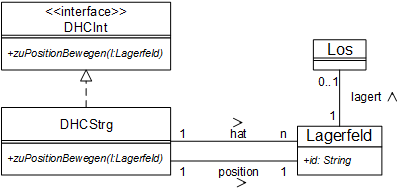
\includegraphics[width=0.6\textwidth]{img/Paketdetails.png}
\caption{\textcolor{blue}{Durch eigene Diagramme ersetzen}}
\label{Paketdetails}
\end{figure}
\subsection{Beschreibung der Klasse \textcolor{blue}{$<$Klassenname$>$}}
\textcolor{blue}{\textit{In diesem Abschnitt sollen die in den Klassendiagrammen enthaltenen Klassen/Schnittstellen weiter beschrieben werden. Hierzu soll zu jeder Klasse eine textuelle Beschreibung erstellt werden.\\\\
Weiterhin soll für wesentliche Operationen der Ablauf in Form von Aktivitätsdiagrammen modelliert werden. Der Lebenszyklus kann durch ein entsprechendes Zustandsdiagramm modelliert werden
}}

\begin{figure}[H]
\centering
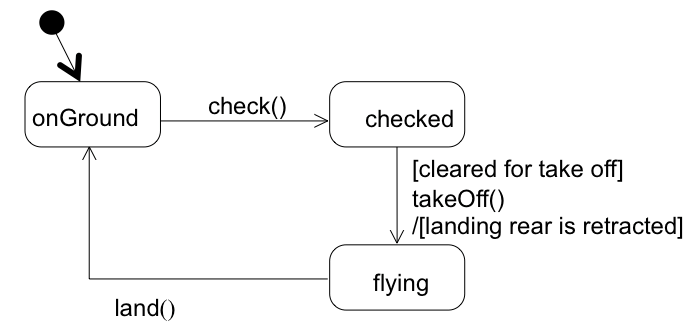
\includegraphics[width=0.6\textwidth]{img/BeschreibungKlasse1.png}
\caption{\textcolor{blue}{Durch eigene Diagramme ersetzen}}
\label{BeschreibungKlasse1}
\end{figure}

\begin{figure}[H]
\centering
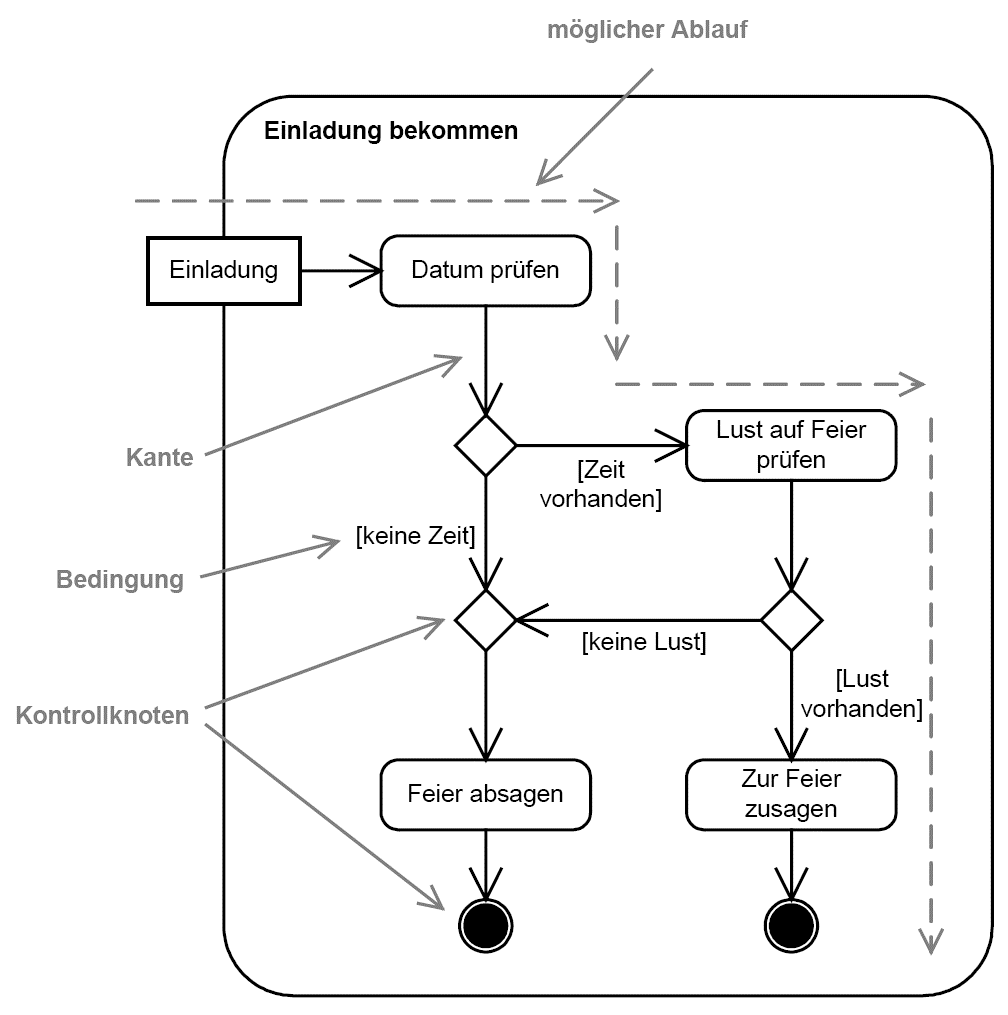
\includegraphics[width=0.6\textwidth]{img/BeschreibungKlasse2.png}
\caption{\textcolor{blue}{Durch eigene Diagramme ersetzen}}
\label{BeschreibungKlasse2}
\end{figure}